\documentclass[11pt,a4paper]{article}

% --- Packages ---
\usepackage[utf8]{inputenc}
\usepackage[T1]{fontenc}
\usepackage{amsmath,amssymb,amsfonts}
\usepackage{graphicx}
\usepackage{booktabs}
\usepackage{hyperref}
\usepackage[margin=1in]{geometry}
\usepackage{microtype}
\usepackage{xcolor}
\usepackage{caption}
\usepackage{subcaption}
\usepackage{float}
\usepackage{enumitem}
\usepackage{natbib}
\bibliographystyle{plainnat}

\hypersetup{
  colorlinks=true,
  linkcolor=blue!60!black,
  citecolor=blue!60!black,
  urlcolor=blue!60!black,
}

% --- Title ---
\title{Hebbian Trace: Persistent and Compositional Memory\\for Frozen Language Models}

\author{
  Andrey Pustovit\\
  Independent Researcher\\
  \texttt{andreyandreevgr@gmail.com}
}

\date{}

\begin{document}
\maketitle

% ============================================================
\begin{abstract}
Large language models are stateless---knowledge acquired during one session is lost when the context resets. We introduce the \emph{Hebbian Trace Module}, a lightweight external memory (${\sim}1$M parameters) that attaches to frozen pretrained LLMs and enables persistent, updatable, cross-session knowledge retention without fine-tuning or retrieval infrastructure. Inspired by hippocampal memory systems, the module combines seven composable, independently ablated mechanisms: sparse pattern separation, Hebbian hetero- and autoassociative storage, dual semantic gating, reconsolidation erasure, complementary learning systems, and replay.

The module transfers with zero-shot generalization across five model scales---GPT-2 Small (124M) through Mistral 7B---spanning three tokenizer families and four architectures. On structured fact tasks, it achieves 98--99\% cross-session recall across 15 sessions with 24 fact types. Autoassociative pattern completion resolves paraphrased queries, improving misaligned accuracy by up to +83 percentage points without degrading aligned retrieval. On LAMA T-REx (2,034 Wikidata facts, 40 relations), cross-context retrieval reaches 81--94\%, exceeding GPT-2's in-context baseline by +50--60pp on a realistic entity vocabulary (${\sim}1{,}100$ unique tokens). Compared to kNN-LM---the closest existing approach for frozen LMs---the trace outperforms by +63pp on cross-context retrieval, where storage and query phrasing differ. Hash-routed trace banks scale capacity to 1,000 simultaneous facts at ${\geq}99\%$ accuracy (128 banks, LLaMA-2 7B) with zero latency overhead. A two-hop retrieval pipeline achieves 100\% end-to-end accuracy on 4,159 HotpotQA bridge questions \emph{without oracle support} (automatic bridge detection from context paragraphs, best-bank scan at retrieval, first-token answer match), maintaining ${\geq}98.7\%$ with up to 15 simultaneous questions via hashed trace banks. An LLM-based extraction pipeline (Flan-T5-small) achieves 94\% F1 on unconstrained text where regex fails entirely. All seven mechanisms compose orthogonally, each targeting an independent bottleneck. Our results suggest that persistent, compositional memory can be added to pretrained language models as a modular plug-in without modifying model weights.
\end{abstract}

% ============================================================
\section{Introduction}

Current large language models \citep{vaswani2017attention,brown2020language} operate as stateless systems---each conversation begins with a blank slate. While in-context learning \citep{brown2020language} allows temporary use of information within a session, this knowledge is lost when the context window resets. Existing solutions each have fundamental limitations: retrieval-augmented generation (RAG) \citep{lewis2020retrieval} requires explicit indexing infrastructure and does not learn or update organically; fine-tuning is computationally expensive, risks catastrophic forgetting, and cannot operate incrementally at inference time; and extended context windows, while accommodating more tokens, still reset between sessions and scale quadratically in compute.

The human brain solves this problem through the hippocampal memory system---a fast-learning complementary structure that rapidly encodes episodic memories, updates them through reconsolidation \citep{nader2000fear}, and operates alongside the slow-learning neocortex \citep{mcclelland1995complementary}. The hippocampus achieves this through a coordinated set of mechanisms: sparse coding in the dentate gyrus minimizes interference between memories \citep{rolls2013mechanisms}, autoassociative networks in CA3 store and retrieve patterns, cholinergic modulation gates encoding versus retrieval modes \citep{hasselmo2006role}, and reconsolidation enables selective updating of existing memories.

We propose the Hebbian Trace Module, an external memory system that translates these hippocampal principles into a computational module attachable to any frozen pretrained language model. Our key contributions are:

\begin{enumerate}[leftmargin=*]
  \item \textbf{A modular persistent memory architecture} comprising seven bio-inspired, independently validated components that compose orthogonally, enabling cross-session knowledge retention, paraphrase resolution, and multi-hop retrieval for frozen LLMs. Hash-routed trace banks extend capacity scaling: with 128 banks, accuracy remains ${\geq}99\%$ through 1,000 simultaneously stored facts on LLaMA-2 7B (vs.\ 9.8\% baseline without banks), with zero measurable latency overhead (${\sim}0.1$ms added to a ${\sim}17$ms forward pass).

  \item \textbf{Architecture-agnostic transfer across five model scales.} Mechanisms developed on a custom transformer (6.4M parameters) transfer to GPT-2 Small (124M), GPT-2 Medium (355M), Phi-2 \citep{javaheripi2023phi} (2.7B), LLaMA-2 7B \citep{touvron2023llama}, and Mistral 7B \citep{jiang2023mistral}---spanning three tokenizer families and four distinct architectures---with zero-shot generalization. Scaling trace heads proportionally to $d_{\text{model}}$ recovers 85\%+ accuracy at $n{=}5$ on LLaMA-2 7B, matching GPT-2 Small.

  \item \textbf{Real-world validation on two public benchmarks.} On the LAMA T-REx benchmark (2,034 Wikidata facts, 40 relations), cross-context trace retrieval achieves 81--94\% accuracy---with automated concept-word assignment matching oracle curation within confidence intervals---exceeding GPT-2's in-context baseline by +50--60pp on a realistic entity vocabulary (1,014--1,107 unique tokens). On HotpotQA \citep{yang2018hotpotqa}, a two-hop trace chain achieves 100\% end-to-end accuracy on 4,159 bridge questions \emph{without oracle support}---bridge entities are identified automatically from context paragraphs (94.6\% agreement with oracle annotations), and best-bank scan retrieval requires no oracle tokens at read time---maintaining ${\geq}98.7\%$ with up to 15 simultaneous question batches (first-token answer match; not comparable to end-to-end QA leaderboard entries). These results validate the trace's multi-hop chaining mechanism on real-world facts, not end-to-end question answering.

  \item \textbf{Autoassociative pattern completion.} A second trace ($\mathbf{T}_{\text{auto}}$) maps variant query vectors to canonical concept vectors, resolving paraphrased questions (+83pp at $n{=}1$) and semantic reformulations (+73pp) without degrading aligned retrieval.

  \item \textbf{Systematic ablation}, isolating the contribution of each component and mapping architectural limitations. We demonstrate +26pp from pattern separation, +46pp from semantic gating, +38pp from reconsolidation erasure, and +83pp from pattern completion on targeted benchmarks.

  \item \textbf{From structured templates to natural interaction.} An LLM-based extraction pipeline (Flan-T5-small) achieves 94\% F1 on unconstrained text where regex fails entirely, and a multi-turn dialogue system demonstrates fact accumulation, updates, and retrieval across conversational turns with 100\% accuracy.
\end{enumerate}

% ============================================================
\section{Related Work}

\textbf{Fast weights and associative memory.}\quad The idea of rapidly updated associative weights has a long history. \citet{ba2016using} proposed fast weights as outer-product accumulations for short-term memory in RNNs. \citet{schlag2021linear} connected linear attention to fast weight memories. Our work extends this line by introducing sparse addressing, gated writing, and selective erasure---mechanisms absent from prior fast weight systems.

\textbf{Modern Hopfield Networks.}\quad \citet{ramsauer2020hopfield} showed that transformer attention can be viewed as a modern Hopfield network with exponential storage capacity. While our Hebbian trace uses similar outer-product storage, we operate as an \emph{external} module with explicit write/read separation, gated storage, and cross-session persistence---properties not present in the attention-as-memory framework.

\textbf{Memory-augmented transformers.}\quad Several works have added external memory to transformers. Neural Turing Machines \citep{graves2014neural} and Memory Networks \citep{sukhbaatar2015end,weston2015memory} introduced differentiable external memory with read/write access. Memorizing Transformers \citep{wu2022memorizing} cache key-value pairs from previous contexts; MemoryLLM \citep{wang2024memoryllm} integrates updatable memory within model parameters. The kNN-LM \citep{khandelwal2020generalization} stores hidden states from a datastore and interpolates nearest-neighbor retrieval with the LM distribution---the closest existing approach to our setting, as it also attaches to frozen models without fine-tuning. Our approach differs in using context-free addressing (the same concept always maps to the same address, regardless of surrounding context), which enables genuine cross-context retrieval where storage and query have different phrasing. We validate this distinction empirically in Section~\ref{sec:knn_comparison}.

\textbf{Sparse distributed memory.}\quad \citet{kanerva1988sparse} introduced sparse high-dimensional addressing for associative memory. Our pattern separation mechanism is a direct computational analog, using random sparse projections to minimize address overlap. The theoretical grounding follows the Johnson--Lindenstrauss lemma \citep{johnson1984extensions}: random projections preserve pairwise distances, while sparsification further decorrelates representations. We demonstrate that this classical technique provides consistent +12--26pp improvements when integrated with modern transformer architectures.

\textbf{Recurrent and linear-attention architectures.}\quad Recent architectures maintain persistent recurrent state across sequences: RWKV \citep{peng2023rwkv} uses linear attention with time-mixing; Mamba \citep{gu2023mamba} employs selective state spaces; RetNet \citep{sun2023retentive} combines recurrence with parallel training. These approaches bake memory into the architecture itself, requiring training from scratch. In contrast, our module attaches to existing frozen models post-hoc, preserving the base model's capabilities while adding persistent memory as a separable component.

\textbf{Compressive and infinite-context memory.}\quad Infini-attention \citep{munkhdalai2024leave} extends transformers with a compressive memory that accumulates key-value states across segments, enabling unbounded context within a single session. Our approach differs in targeting \emph{cross-session} persistence---memory survives context resets---and in using Hebbian learning rather than gradient-based memory updates, enabling operation on fully frozen models.

\textbf{Complementary Learning Systems.}\quad \citet{mcclelland1995complementary} proposed that memory relies on complementary fast (hippocampal) and slow (neocortical) learning systems. Our per-head decay specialization (Section~\ref{sec:cls}) implements this principle within the trace module, with fast-decay heads tracking recent updates and slow-decay heads maintaining stable long-term associations.

% ============================================================
\section{Architecture}

The Hebbian Trace Module attaches to a frozen pretrained language model as an external memory. It intercepts token embeddings for addressing, stores associations via Hebbian learning \citep{hebb1949organization}, and injects retrieved information into the model's output logits. Figure~\ref{fig:architecture} shows the complete architecture.

\begin{figure}[t]
  \centering
  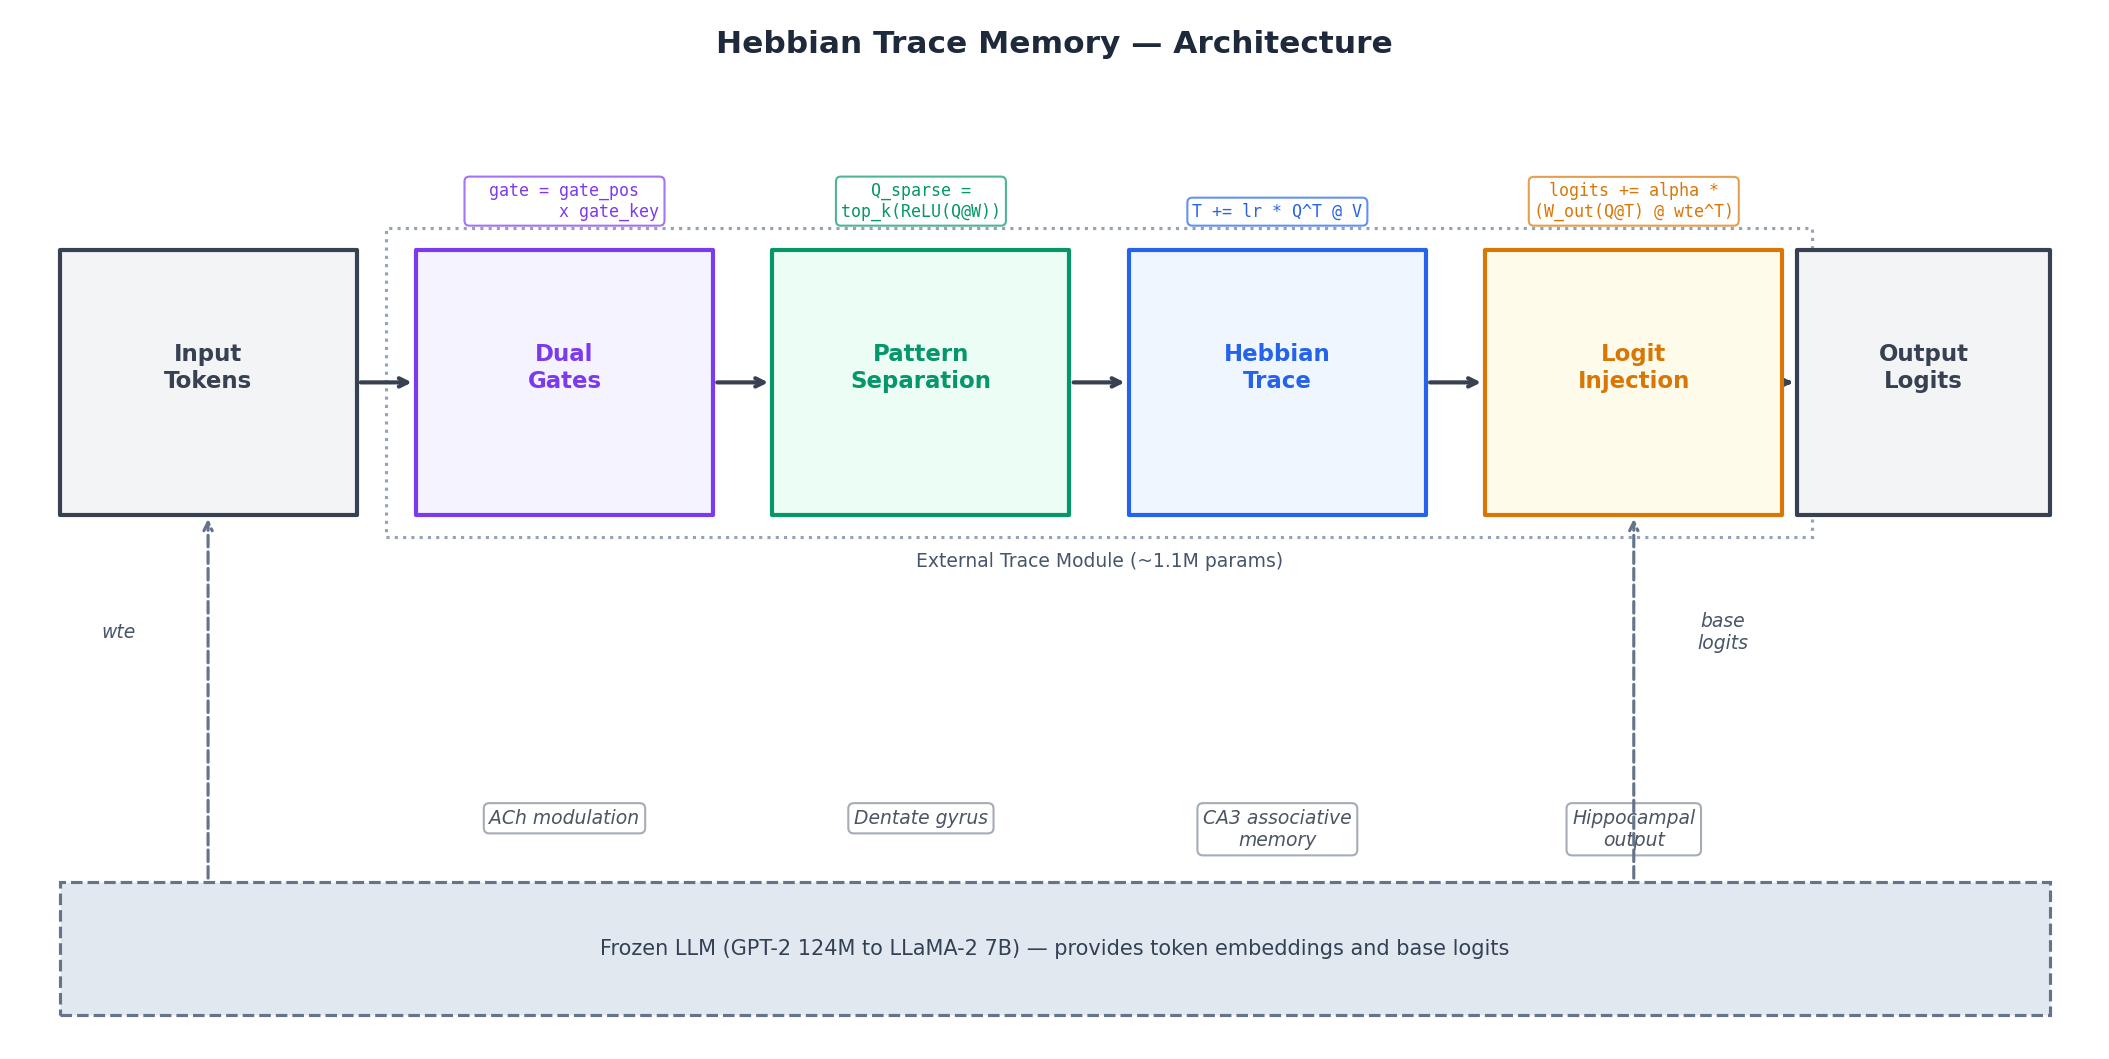
\includegraphics[width=\textwidth]{figures/architecture.png}
  \caption{Architecture of the Hebbian Trace Module attached to frozen GPT-2. Input token embeddings pass through dual gates (cholinergic modulation analog), pattern separation (dentate gyrus), Hebbian trace storage (CA3), and logit injection. The frozen model provides embeddings and base logits; the trace module (${\sim}1.1$M parameters) operates entirely in the logit space.}
  \label{fig:architecture}
\end{figure}

\subsection{Core Mechanism: Hebbian Associative Trace}

The trace stores key-value associations in a matrix $\mathbf{T}_v \in \mathbb{R}^{d \times d}$ (per attention head) via rank-1 Hebbian updates:
\begin{equation}
  \mathbf{T}_v \leftarrow \gamma \cdot \mathbf{T}_v + \eta \cdot \mathbf{Q}_{\text{store}}^\top \cdot \mathbf{V}_{\text{store}}
  \label{eq:hebbian_update}
\end{equation}
where $\gamma$ is a decay factor, $\eta$ is a learning rate, $\mathbf{Q}_{\text{store}}$ is the key vector derived from the concept word's embedding, and $\mathbf{V}_{\text{store}}$ is the value vector derived from the entity embedding. Retrieval computes:
\begin{equation}
  \mathbf{V}_{\text{retrieved}} = \mathbf{Q}_{\text{addr}} \cdot \mathbf{T}_v
  \label{eq:retrieval}
\end{equation}
The retrieved values are projected back to model dimension and injected as a logit bias:
\begin{equation}
  \text{logits} \leftarrow \text{logits} + \alpha \cdot \mathbf{W}_{\text{out}}(\mathbf{V}_{\text{retrieved}}) \cdot \mathbf{W}_{\text{embed}}^\top
  \label{eq:logit_injection}
\end{equation}
where $\mathbf{W}_{\text{embed}}$ is the model's token embedding matrix (weight-tied with the language model head), and $\alpha$ controls injection strength. This logit-space injection directly biases predictions toward stored entities without requiring injection into intermediate residual streams.

\textbf{Addressing via token embeddings.}\quad Both $\mathbf{Q}$ and $\mathbf{V}$ are derived from the model's token embeddings (wte) through learned projections: $\mathbf{Q} = \mathbf{W}_{\text{proj}}(\text{LN}(\text{wte}(\text{token})))$, $\mathbf{V} = \mathbf{W}_{\text{val}}(\text{wte}(\text{token}))$. Using raw embeddings rather than contextual hidden states provides context-free addressing---the same concept word produces the same address regardless of surrounding context, enabling cross-session retrieval.

\subsection{Pattern Separation (Dentate Gyrus Analog)}
\label{sec:pattern_sep}

In the hippocampus, the dentate gyrus creates sparse, decorrelated representations from cortical input, minimizing interference between similar memories. We implement this as a frozen random sparse expansion:
\begin{equation}
  \mathbf{Q}_{\text{sparse}} = \text{TopK}(\text{ReLU}(\mathbf{W}_{\text{expand}} \cdot \mathbf{Q}),\, k)
  \label{eq:pattern_sep}
\end{equation}
where $\mathbf{W}_{\text{expand}} \in \mathbb{R}^{(f \cdot d) \times d}$ is a frozen random matrix (expansion factor $f$, typically $8\times$), and $\text{TopK}$ retains only the $k$ largest activations (typically 16). This transforms dense $\mathbf{Q}$ vectors into sparse codes where different concepts activate nearly non-overlapping dimensions.

The expansion matrix $\mathbf{W}_{\text{expand}}$ receives no gradient and remains random---directly analogous to the largely random mossy fiber projections from dentate gyrus to CA3. At expansion $8\times$ with $k{=}16$ on MiniGPT ($d_{\text{head}}{=}32$, yielding 6.25\% sparsity), mean cosine similarity between concept Q-vectors drops from 0.477 to 0.308, with intersection-over-union of 0.173.

\textbf{Empirical impact.}\quad Pattern separation consistently provides +9--26pp accuracy improvement across all experimental settings---from custom transformers to pretrained GPT-2, from single facts to multi-session scenarios (see Figure~\ref{fig:ablation}).

\subsection{Dual Semantic Gating (Cholinergic Modulation Analog)}

In the hippocampus, acetylcholine modulates the transition between encoding and retrieval modes, controlling what information enters long-term storage. We implement this through two complementary gates:

\textbf{Position gate} ($g_{\text{pos}}$): A learned linear classifier on token embeddings that identifies \emph{where} linking tokens occur---positions that signal key-value relationships (e.g., ``is'', ``in'', ``at''):
\begin{equation}
  g_{\text{pos}} = \sigma(\mathbf{W}_{\text{gate}} \cdot \text{wte}(\text{token}))
  \label{eq:pos_gate}
\end{equation}

\textbf{Semantic gate} ($g_{\text{key}}$): A learned linear classifier that evaluates \emph{whether} the concept word at the linking position is worth storing:
\begin{equation}
  g_{\text{key}} = \sigma(\mathbf{W}_{\text{gate\_key}} \cdot \text{wte}(\text{token}))
  \label{eq:sem_gate}
\end{equation}

The combined gate is their product: $g_{\text{combined}} = g_{\text{pos}}[\text{link}] \cdot g_{\text{key}}[\text{concept}]$. This dual gating enables paragraph-level storage: the model processes natural text containing both relevant facts and irrelevant filler, storing only meaningful associations.

\textbf{Discovery without supervision.}\quad Both gates are trained purely through cross-context retrieval loss---no explicit labels for linking tokens or concept words. The position gate achieves $167\times$ selectivity between linking and non-linking tokens. The semantic gate achieves $6.4\times$ selectivity between fact concepts (avg${=}0.401$) and filler concepts (avg${=}0.063$). Together, they reduce the accuracy gap between clean and noisy input from 44pp to 2.6pp.

\subsection{Reconsolidation Erasure}

Memory reconsolidation in neuroscience refers to the process where retrieved memories become labile and can be modified or erased \citep{nader2000fear}. We implement selective erasure for fact updates:
\begin{align}
  \hat{\mathbf{Q}} &= \mathbf{Q} / \|\mathbf{Q}\|_2 \label{eq:q_norm} \\
  \mathbf{V}_{\text{old}} &= \hat{\mathbf{Q}} \cdot \mathbf{T}_v \label{eq:retrieve_old} \\
  \mathbf{T}_v &\leftarrow \mathbf{T}_v - \eta_{\text{erase}} \cdot \hat{\mathbf{Q}}^\top \cdot \mathbf{V}_{\text{old}} \label{eq:erase} \\
  \mathbf{T}_v &\leftarrow \mathbf{T}_v + \eta \cdot \mathbf{Q}^\top \cdot \mathbf{V}_{\text{new}} \label{eq:write_new}
\end{align}
$L_2$ normalization of $\mathbf{Q}$ before erasure is critical---without it, the erasure magnitude scales with $\|\mathbf{Q}\|^2$, causing catastrophic over-erasure. With normalized $\mathbf{Q}$, erasure precisely targets the stored association at that address.

\textbf{Impact on fact updates.}\quad In a 10-session scenario with 5 fact updates, erasure improves update accuracy from 61\% to 99\% (+38pp). Trace norm decreases during updates ($11.0 \to 8.6$), confirming that erasure actively cleans the trace rather than merely overwriting.

\subsection{Complementary Learning Systems: Per-Head Specialization}
\label{sec:cls}

Inspired by CLS theory \citep{mcclelland1995complementary}, we assign different temporal dynamics to different attention heads within the trace. ``Slow'' heads (high decay, $\gamma{=}0.99$) maintain stable long-term associations, while ``fast'' heads (low decay, $\gamma{=}0.90$) quickly adapt to updated information:
\begin{equation}
  \mathbf{T}_v^h \leftarrow \gamma_h \cdot \mathbf{T}_v^h + \eta \cdot \mathbf{Q}^\top \cdot \mathbf{V}
  \label{eq:cls}
\end{equation}
This specialization is irrelevant when all facts are equally important (confirmed in ablation), but becomes critical for fact update tasks: split-decay heads improve overall accuracy by +7.4pp compared to uniform decay, specifically by reducing old-value interference from 28.5\% to 16.2\%.

\subsection{Autoassociative Pattern Completion (CA3 Analog)}
\label{sec:tauto}

The hippocampal CA3 region functions as both a heteroassociative memory (mapping cues to stored patterns) and an autoassociative memory (completing partial or degraded cues to full patterns) \citep{rolls2013mechanisms}. Our heteroassociative trace $\mathbf{T}_v$ maps concept Q-vectors to entity V-vectors. We add a complementary autoassociative trace $\mathbf{T}_{\text{auto}}$ that maps variant Q-vectors to canonical concept Q-vectors:
\begin{equation}
  \mathbf{T}_{\text{auto}} \leftarrow \mathbf{T}_{\text{auto}} + \eta \cdot \mathbf{Q}_{\text{variant}}^\top \cdot \mathbf{Q}_{\text{concept}}
  \label{eq:tauto_write}
\end{equation}
Unlike $\mathbf{T}_v$, updates to $\mathbf{T}_{\text{auto}}$ are purely additive (no decay)---these are static linguistic mappings, not episodic memories. Retrieval proceeds in two steps:
\begin{align}
  \mathbf{Q}_{\text{corrected}} &= \mathbf{Q}_{\text{variant}} \cdot \mathbf{T}_{\text{auto}} \label{eq:tauto_read} \\
  \text{logits}_{\text{completion}} &= \alpha_c \cdot \mathbf{W}_{\text{out}}(\mathbf{Q}_{\text{corrected}} \cdot \mathbf{T}_v) \cdot \mathbf{W}_{\text{embed}}^\top \label{eq:completion_logits}
\end{align}
where $\alpha_c$ is the completion channel strength (optimal at 0.3). The completion channel operates in parallel with the standard retrieval path, and their logits are summed. When $\mathbf{T}_{\text{auto}}$ contains no relevant mapping, $\mathbf{Q}_{\text{corrected}}$ is near-zero and contributes negligible signal.

\subsection{Multi-Hop Chain Retrieval}
\label{sec:multihop}

Standard trace retrieval handles single-hop queries: Q(concept) $\to$ $\mathbf{T}_v$ $\to$ entity. Multi-hop retrieval requires chaining: ``Where does John live?'' $\to$ Paris $\to$ ``What country is Paris in?'' $\to$ France. We implement this with zero new parameters via a direct retrieval pipeline:
\begin{align}
  \text{token}_1 &= \arg\max\, \mathbf{W}_{\text{out}}(\mathbf{Q}_{\text{addr}} \cdot \mathbf{T}_v) \cdot \mathbf{W}_{\text{embed}}^\top \label{eq:hop1} \\
  \mathbf{Q}_2 &= \mathbf{W}_{\text{proj}}(\text{LN}(\text{wte}(\text{token}_1))) \label{eq:reencode} \\
  \text{token}_2 &= \arg\max\, \mathbf{W}_{\text{out}}(\mathbf{Q}_{2,\text{addr}} \cdot \mathbf{T}_v) \cdot \mathbf{W}_{\text{embed}}^\top \label{eq:hop2}
\end{align}
Hop-1 retrieves an intermediate entity, decodes it via argmax over the embedding matrix, re-encodes it as a new query vector, and performs a second trace lookup. Both hops use the same trace $\mathbf{T}_v$---chain links are stored as entity-as-concept associations (e.g., Q(``Paris'') $\to$ V(``France'')). This \texttt{retrieve\_direct} operation bypasses the frozen LM entirely, using pure trace signal without $\alpha$-scaled LM logits, which we show matches standard forward-pass retrieval in accuracy (Section~\ref{sec:multihop_exp}).

% ============================================================
\section{Experimental Validation}

We validate the architecture through systematic experiments across five model scales and four architectures, following a progression from individual components to multi-hop retrieval on a real benchmark.

\subsection{Development Platform: Custom Transformer (MiniGPT)}

Initial development used a custom 6.4M-parameter transformer ($d_{\text{model}}{=}128$, 4--8 heads, 176-token vocabulary) trained on synthetic key-value association tasks. This controlled setting allowed rapid iteration on architectural choices.

Key findings from ablation studies are summarized in Table~\ref{tab:ablation} and visualized in Figure~\ref{fig:ablation}.

\begin{table}[t]
  \centering
  \caption{Component ablation on MiniGPT. Each mechanism targets an independent bottleneck, validated on the specific task where that bottleneck is binding. Effects compose orthogonally.}
  \label{tab:ablation}
  \begin{tabular}{@{}llll@{}}
    \toprule
    Component & Task / Condition & Effect ($n{=}10$) & Mechanism \\
    \midrule
    Pattern separation (\S\ref{sec:pattern_sep}) & Cross-context retrieval & +9.3pp & Sparse Q reduces interference \\
    Adaptive alpha & Hebbian / cross-context & +16pp / +2pp & Score trace normalization \\
    CLS decay (\S\ref{sec:cls}) & Fact updates (10 sessions) & +7.4pp overall & Fast/slow head specialization \\
    Selective erasure (\S3.3) & Fact updates (10 sessions) & +11.7pp overall & Anti-Hebbian old-value removal \\
    Concept injection & Tier~2 templates & +90pp & Semantic Q override \\
    Dual gates (\S3.2) & Noisy paragraphs & +46pp & Semantic filtering of storage \\
    \bottomrule
  \end{tabular}
\end{table}

\begin{figure}[t]
  \centering
  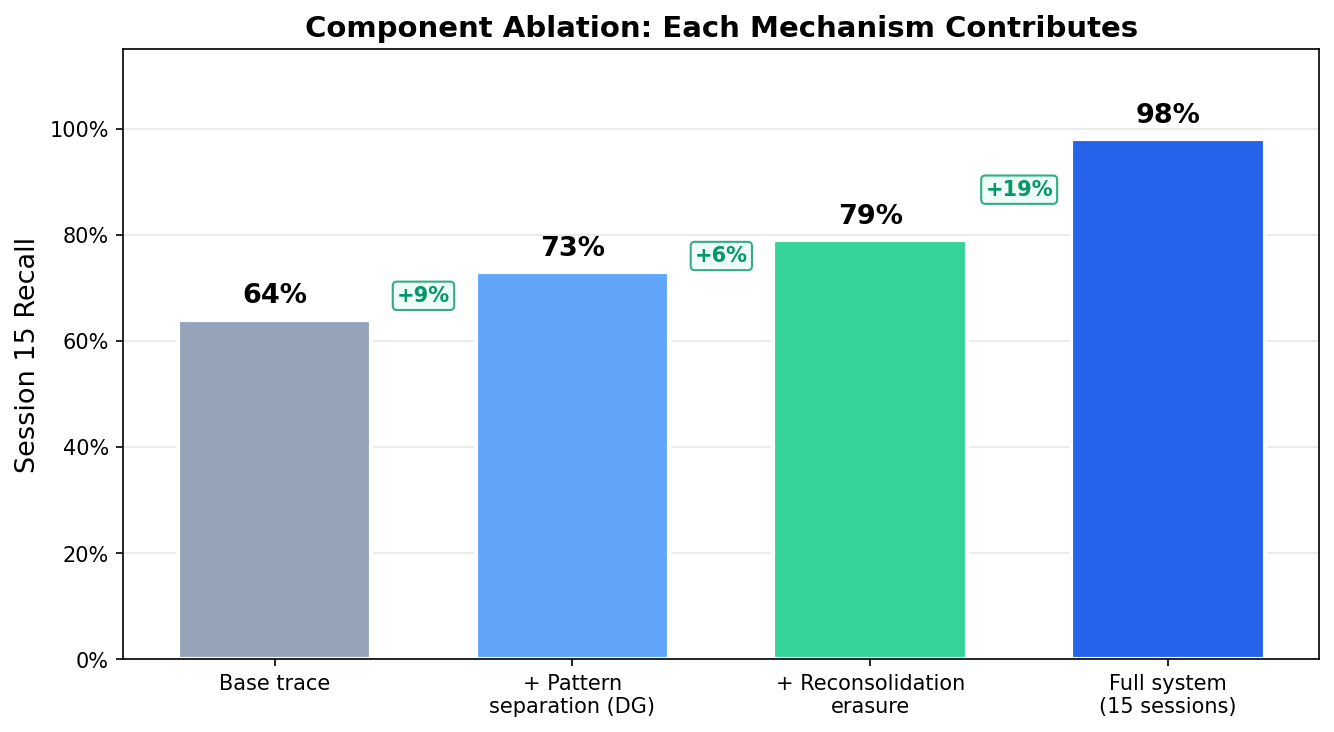
\includegraphics[width=0.75\textwidth]{figures/ablation_chart.png}
  \caption{Cumulative contribution of each mechanism to session-15 recall in the multi-session flagship experiment. Each component addresses an independent bottleneck, and their effects are approximately additive.}
  \label{fig:ablation}
\end{figure}

\subsection{Transfer to Pretrained GPT-2}

We attached the trace module to frozen GPT-2 Small \citep{radford2019language} (124M parameters) as an external memory with ${\sim}1.1$M trainable parameters ($\mathbf{W}_{\text{proj}}$, $\mathbf{W}_{\text{val}}$, $\mathbf{W}_{\text{out}}$, $\mathbf{W}_{\text{gate}}$, $\mathbf{W}_{\text{gate\_key}}$).

\textbf{Zero-shot proof of concept.}\quad With random projections and zero fine-tuning, the trace achieves 100\% cross-context recall at $n{=}1$ (vs.\ 4\% baseline) and 84.1\% at $n{=}7$ with pattern separation (Figure~\ref{fig:cross_context}). This demonstrates that GPT-2's embedding space is sufficiently structured for Hebbian association without learned projections.

\textbf{Pattern separation transfers identically.}\quad The same +12pp improvement magnitude observed on MiniGPT appears on GPT-2, confirming the mechanism's model-independence. Transfer to GPT-2 Medium (355M parameters) shows consistent improvements across model scales (Figure~\ref{fig:model_scaling}).

\textbf{Alpha calibration.}\quad Optimal injection strength shifts from $\alpha{=}0.1$ (MiniGPT) to $\alpha{=}0.5$ (GPT-2), reflecting the larger model's higher confidence in its own predictions requiring stronger trace signal.

\textbf{Cross-architecture transfer: Phi-2 (2.7B).}\quad To test architecture-agnostic generalization, we attached the trace module to Microsoft Phi-2 \citep{javaheripi2023phi} (2.7B parameters)---a fundamentally different architecture using parallel attention, rotary position embeddings, and a CodeGen tokenizer. The transfer is fully zero-shot: no gate weights are loaded (incompatible $d_{\text{model}}$: 768 vs.\ 2560), and all projections are randomly initialized. Only the hardcoded linking-token mask is used.

With $\alpha{=}50$ and pattern separation ($8\times$, $k{=}16$), Phi-2 achieves 100\% at $n{=}1$ and 98.4\% at $n{=}5$ (Table~\ref{tab:scaling}). Notably, Phi-2 \emph{exceeds} GPT-2 Small at $n{\geq}5$ by +7--8pp, suggesting that larger embedding spaces provide better-separated Q-vectors for Hebbian storage. The optimal $\alpha$ is $50\times$ higher than GPT-2's, consistent with the larger model's logit scale.

\textbf{Scaling to 7B: LLaMA-2 and Mistral.}\quad We further tested transfer to LLaMA-2 7B \citep{touvron2023llama} and Mistral 7B \citep{jiang2023mistral}---both SentencePiece-tokenized, with rotary embeddings and grouped-query attention. As with Phi-2, transfer is fully zero-shot with random projections.

With the default trace configuration ($H{=}8$, $d_{\text{trace}}{=}64$), both 7B models achieved ${\sim}95$--97\% at $n{=}1$ but degraded to ${\sim}67$--70\% at $n{=}5$ (Table~\ref{tab:scaling}). Diagnosis revealed that the bottleneck is trace dimensionality: the random $\mathbf{W}_{\text{out}}$ projects from $H \times d_{\text{trace}} = 512$ dimensions to $d_{\text{model}}{=}4096$---an 8:1 expansion that disperses the trace signal across too many dimensions. Increasing the number of trace heads to $H{=}32$ (total trace dimension $32 \times 64 = 2048$, ratio 1:2 vs.\ $d_{\text{model}}$) recovers accuracy on LLaMA-2: 100\% at $n{=}1$, 94\% at $n{=}3$, and 85.6\% at $n{=}5$---matching GPT-2 Small (Table~\ref{tab:scaling}). The same head-scaling fix does not improve Mistral (67.6\% at $n{=}5$), suggesting a model-specific embedding geometry incompatibility; Mistral's 100$\times$ higher optimal $\alpha$ relative to LLaMA-2 (same $d_{\text{model}}$) points to fundamentally different embedding structure rather than a trace architecture limitation.

\begin{table}[t]
  \centering
  \caption{Cross-architecture transfer across five model scales and three tokenizer families (BPE, CodeGen, SentencePiece). All configurations use pattern separation ($8\times$, $k{=}16$), random projections, and linking-token mask (no trained gates). 50--100 episodes per condition.}
  \label{tab:scaling}
  \begin{tabular}{@{}lrrrccccc@{}}
    \toprule
    Model & Params & $d_{\text{model}}$ & $\alpha$ & Trace $H \times d$ & $n{=}1$ & $n{=}3$ & $n{=}5$ & $n{=}7$ \\
    \midrule
    GPT-2 Small & 124M & 768 & 0.5 & $8 \times 64$ & \textbf{100\%} & 89.7\% & 85.4\% & 82.0\% \\
    GPT-2 Medium & 355M & 1024 & 0.5 & $8 \times 64$ & \textbf{100\%} & 72.7\% & 70.4\% & 69.6\% \\
    Phi-2 & 2.7B & 2560 & 50 & $8 \times 64$ & \textbf{100\%} & 99.3\% & \textbf{98.4\%} & 92.9\% \\
    \addlinespace
    Mistral 7B & 7B & 4096 & 1000 & $8 \times 64$ & 95\% & 74.3\% & 67.4\% & --- \\
    Mistral 7B & 7B & 4096 & 1000 & $32 \times 64$ & 96\% & 73.3\% & 67.6\% & --- \\
    \addlinespace
    LLaMA-2 7B & 7B & 4096 & 10 & $8 \times 64$ & 97\% & 73.7\% & 69.8\% & --- \\
    LLaMA-2 7B & 7B & 4096 & 20 & $32 \times 64$ & \textbf{100\%} & \textbf{94.0\%} & \textbf{85.6\%} & --- \\
    \bottomrule
  \end{tabular}
\end{table}

Counterfactual evaluation further tests whether the trace can override pretrained knowledge with incorrect facts (e.g., ``the capital of France is Berlin''). At $n{=}1$, GPT-2 Small overrides its own prior 96\% of the time, LLaMA-2 achieves 64\%, and Mistral 70\%---confirming that the trace can suppress even 7B-scale priors, though larger models resist more strongly (Table~\ref{tab:counterfactual}).

\begin{table}[t]
  \centering
  \caption{Counterfactual override: trace accuracy on facts contradicting pretrained knowledge. ``Prior'' shows the model's pre-existing accuracy on the counterfactual answer (expected ${\sim}0\%$). 50 episodes.}
  \label{tab:counterfactual}
  \begin{tabular}{@{}lrcccc@{}}
    \toprule
    Model & Params & Prior & Trace $n{=}1$ & Trace $n{=}3$ & Trace $n{=}5$ \\
    \midrule
    GPT-2 Small & 124M & 0\% & \textbf{96\%} & 90\% & 80.4\% \\
    GPT-2 Medium & 355M & 0\% & 66\% & 59.3\% & 56.4\% \\
    LLaMA-2 7B & 7B & 4\% & 64\% & 55.3\% & 51.6\% \\
    Mistral 7B & 7B & 0\% & 70\% & 52.7\% & 48.4\% \\
    \bottomrule
  \end{tabular}
\end{table}

\begin{figure}[t]
  \centering
  \begin{subfigure}[t]{0.48\textwidth}
    \centering
    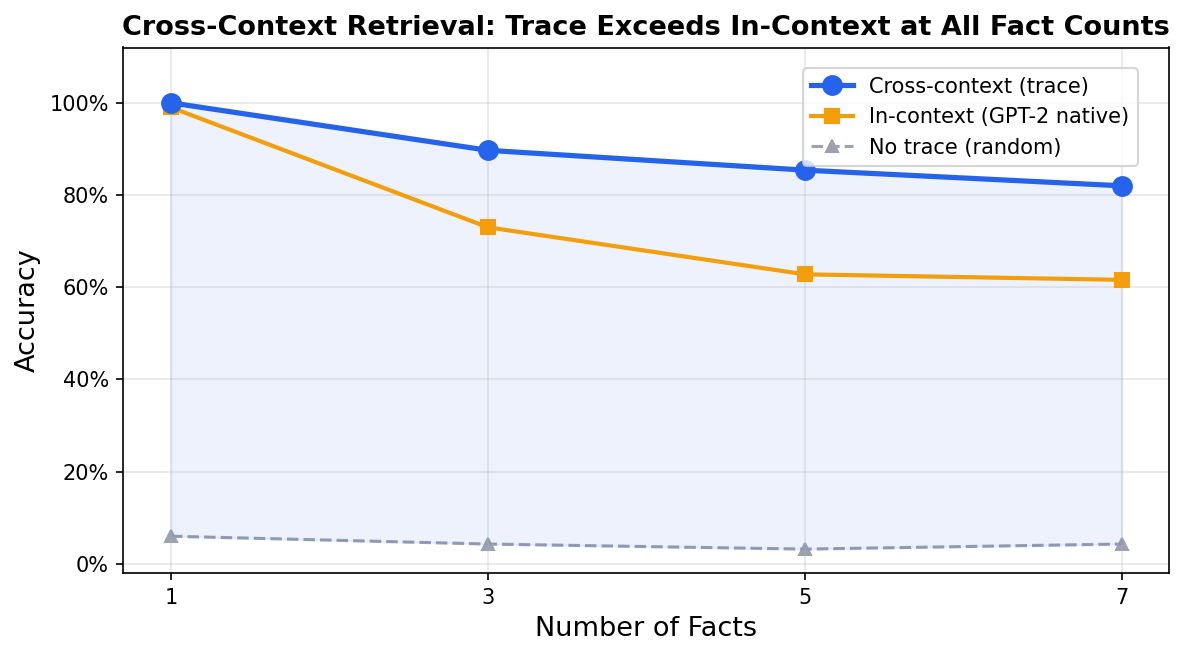
\includegraphics[width=\textwidth]{figures/cross_context.png}
    \caption{Cross-context retrieval accuracy at varying fact counts. The trace exceeds both GPT-2's in-context baseline and kNN-LM at all fact counts (+63pp vs.\ kNN-LM at $n{=}5$).}
    \label{fig:cross_context}
  \end{subfigure}
  \hfill
  \begin{subfigure}[t]{0.48\textwidth}
    \centering
    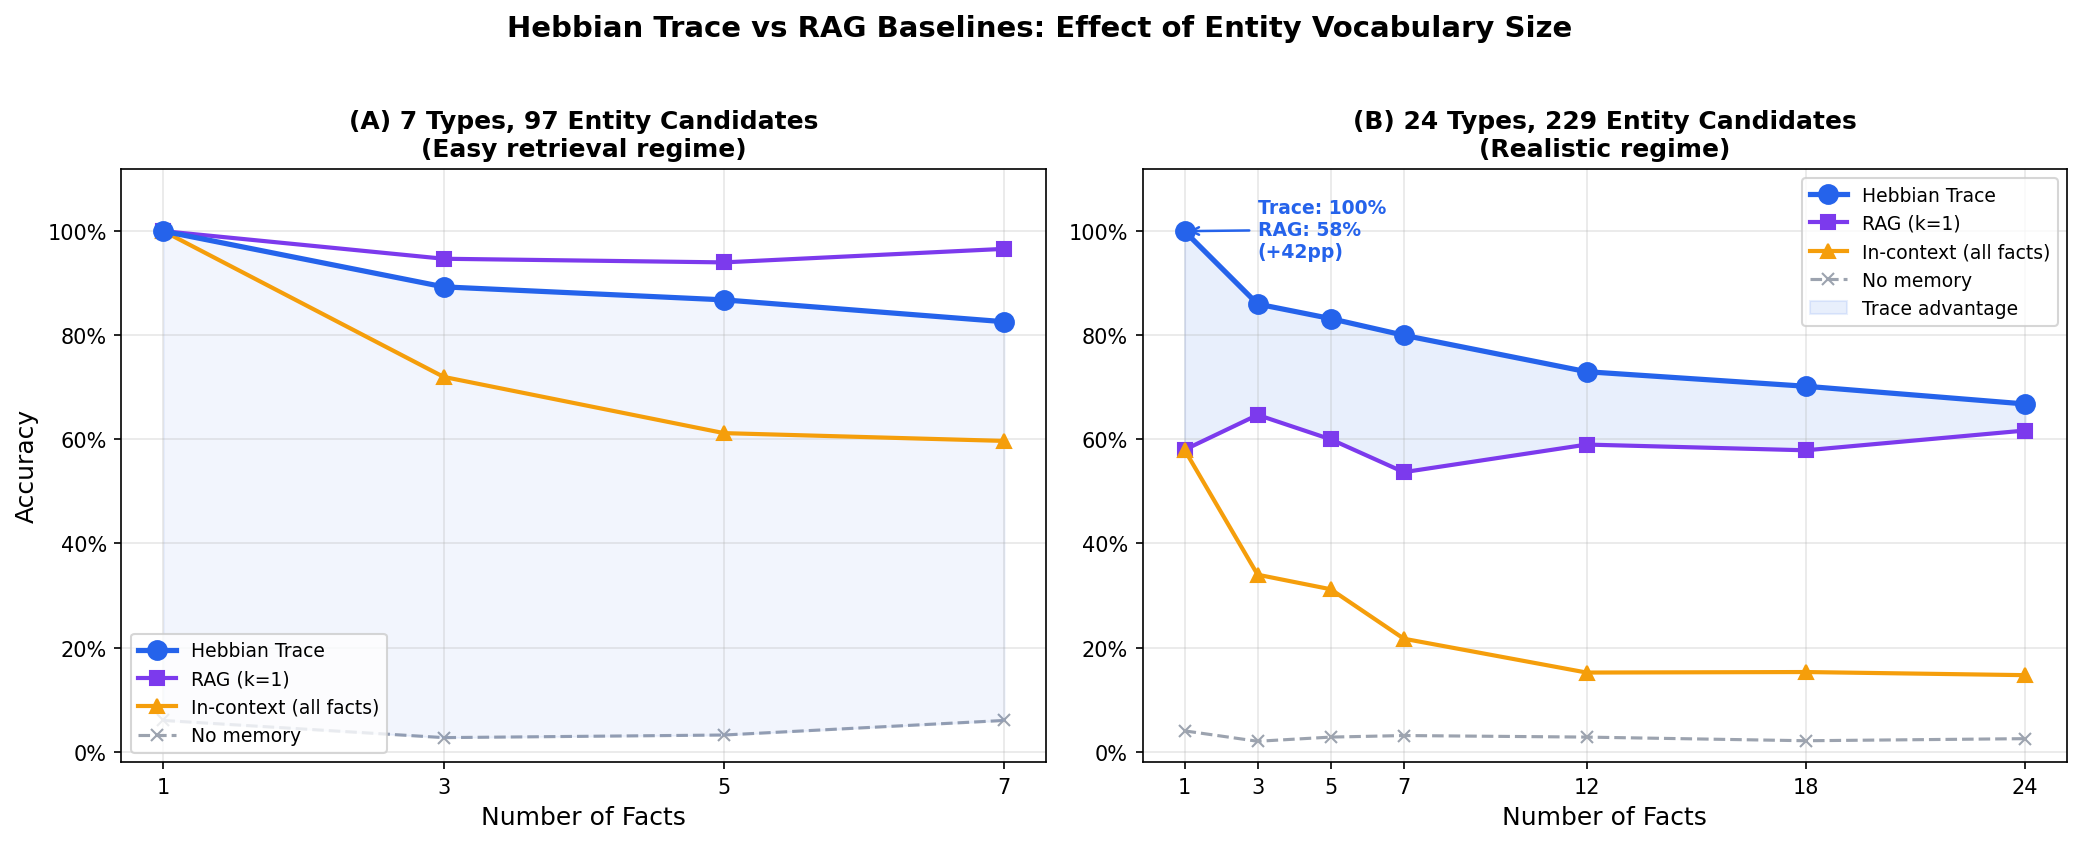
\includegraphics[width=\textwidth]{figures/rag_comparison.png}
    \caption{Comparison with RAG-Oracle (perfect retrieval upper bound). In the easy 7-type regime, Oracle RAG exceeds the trace; in the realistic 24-type regime (229 entity candidates), the trace outperforms Oracle RAG by up to +42pp, as concept-addressed retrieval is phrasing-invariant while RAG degrades with vocabulary size.}
    \label{fig:rag}
  \end{subfigure}
  \caption{Cross-context retrieval performance on GPT-2 Small.}
  \label{fig:retrieval}
\end{figure}

\begin{figure}[t]
  \centering
  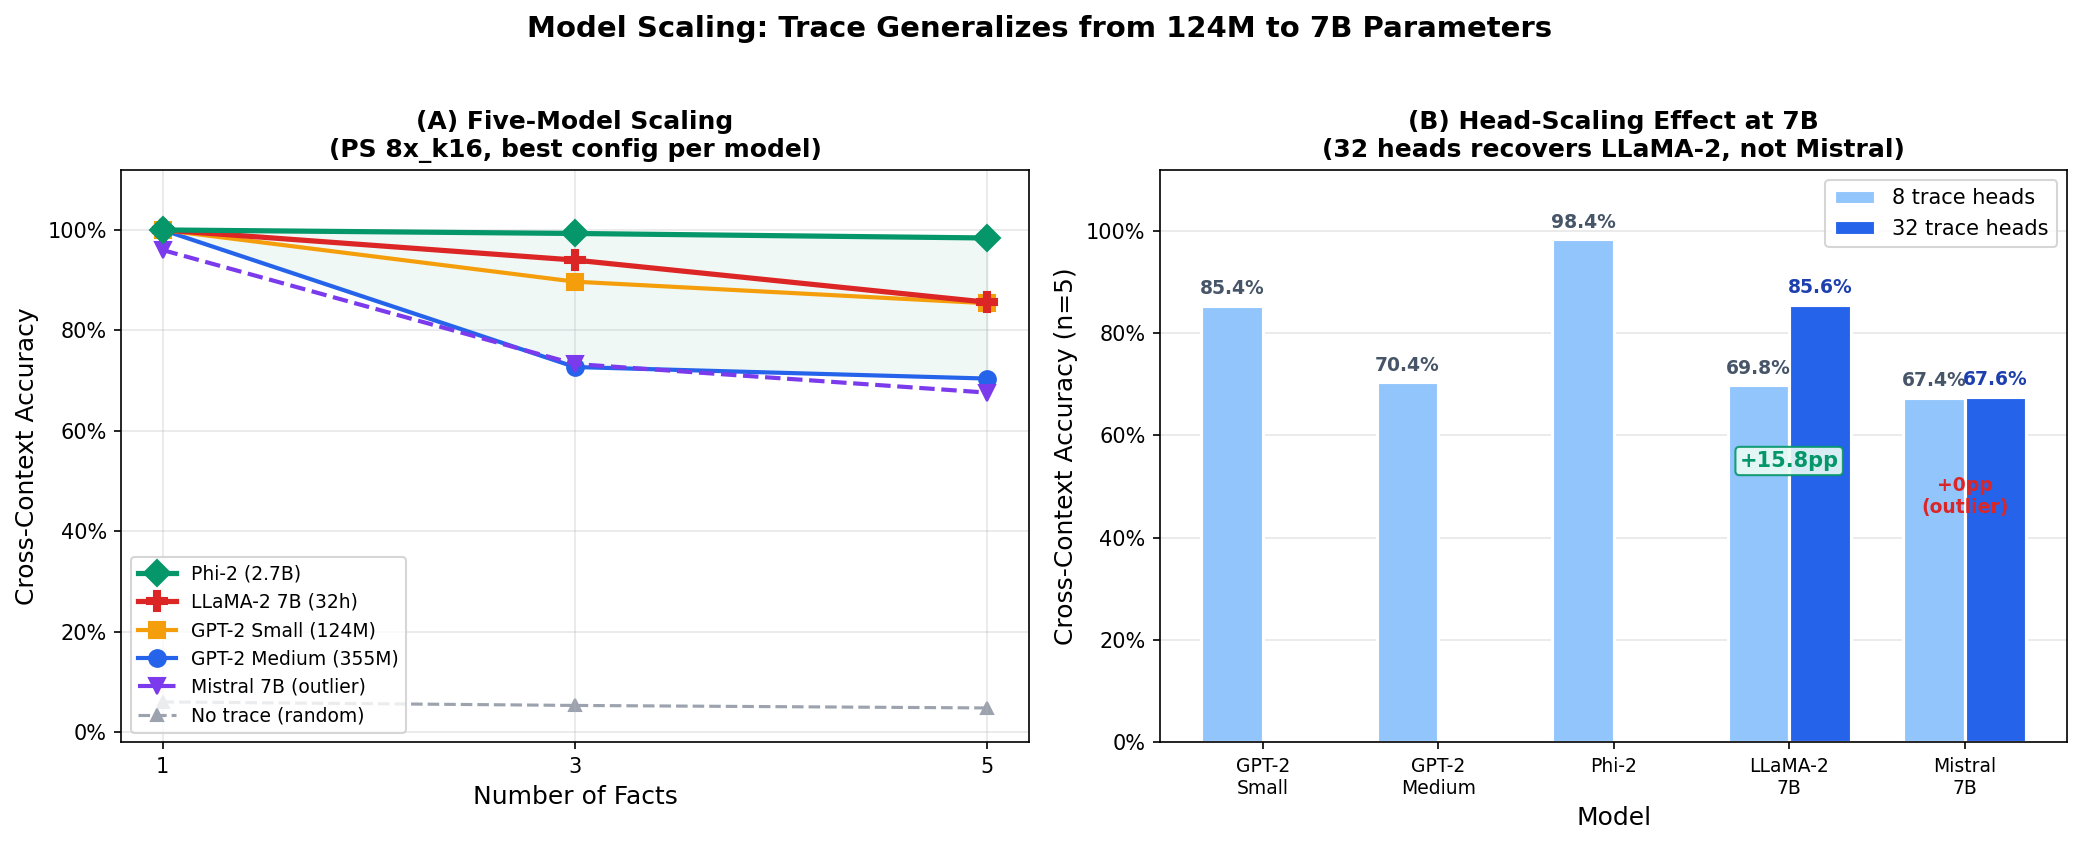
\includegraphics[width=\textwidth]{figures/model_scaling.png}
  \caption{Transfer across model scales. (A)~Cross-context retrieval generalizes from GPT-2 Small (124M) to Medium (355M) with consistent +3--4pp improvements. (B)~Pattern separation provides comparable gains on both model sizes, confirming model-independence. Extended scaling results across five architectures are in Table~\ref{tab:scaling}.}
  \label{fig:model_scaling}
\end{figure}

\subsection{Learned Storage Gating}

Replacing the handcrafted linking-token mask with a learned gate (769 parameters) achieves equivalent accuracy while discovering the same token-level structure without supervision. Adding the semantic gate (769 additional parameters) reduces the noisy-paragraph accuracy gap from 44pp to 7.8pp, and to 2.6pp when combined with pattern separation.

\subsection{Architectural Limitations}
\label{sec:arch_limitations}

Systematic diagnostic reveals three ceiling effects of context-free addressing:

\begin{table}[h]
  \centering
  \caption{Architectural limitations of context-free addressing.}
  \label{tab:limitations}
  \begin{tabular}{@{}lll@{}}
    \toprule
    Limitation & Impact & Root cause \\
    \midrule
    Shift-1 addressing & $-60$pp on paraphrased questions & Retrieval depends on exact token position \\
    Context-free Q & $-48$pp with distractors (70\% confusion) & Cannot distinguish ``My name'' from ``Alice's name'' \\
    Q-collision & $-29$pp with repeated fact types & Same concept word $\to$ same address \\
    \bottomrule
  \end{tabular}
\end{table}

These limitations motivate context-enriched addressing (Section~\ref{sec:context_enriched}) and define clear targets for future work.

\subsection{Context-Enriched Addressing}
\label{sec:context_enriched}

Blending context-free and contextual $\mathbf{Q}$ via $\mathbf{Q} = \mathbf{Q}_{\text{base}} + \beta \cdot \mathbf{W}_{\text{ctx}}(\mathbf{h})$ reveals a Pareto trade-off: increasing $\beta$ improves distractor discrimination at the cost of cross-session stability. Contrastive training of $\mathbf{W}_{\text{ctx}}$ reduces confusion from 74.7\% to 28.0\% at $\beta{=}0.5$, while cross-context alignment loss further improves the frontier.

\subsection{Flagship Result: Multi-Session Persistent Memory}
\label{sec:flagship}

The complete system demonstrates persistent memory across sessions.

\textbf{Setup.}\quad Frozen GPT-2 Small + trace module ($\alpha{=}0.5$, 8 heads, $d_{\text{trace}}{=}64$, pattern separation $8\times/k{=}16$). 24 fact types, 15 sessions, 3--5 facts per session introduced in natural paragraphs with filler sentences.

\begin{table}[t]
  \centering
  \caption{Flagship multi-session results. The trace module maintains ${\geq}98\%$ recall across 15 sessions with fact updates and noisy paragraph input.}
  \label{tab:flagship}
  \begin{tabular}{@{}ll@{}}
    \toprule
    Metric & Value \\
    \midrule
    Total facts stored & 24 \\
    Sessions & 15 (3--5 facts introduced per session) \\
    Mean recall across sessions & 98.6\% \\
    Session 15 recall (all 24 facts active) & 98\% \\
    Single-pass recall at $n{=}24$ & 94.4\% (CI: 92.3--96.5\%) \\
    Retention drop over 15 sessions & $\leq$2pp \\
    Update accuracy (with erasure) & 99\% \\
    Noisy paragraph filtering & 98--99\% (all filler modes) \\
    Trainable parameters & ${\sim}1.1$M (0.9\% of GPT-2) \\
    \bottomrule
  \end{tabular}
\end{table}

\textbf{Incremental vs.\ single-pass.}\quad The 4.2pp gap between incremental multi-session recall (98\%) and single-pass capacity at $n{=}24$ (94.4\%) reflects two effects: (1)~incremental introduction allows the trace to consolidate associations with less mutual interference, and (2)~the decay factor progressively attenuates older entries, which is less harmful when entries are refreshed across sessions via cumulative replay.

The dual gate achieves $103\times$ selectivity between fact and filler sentences, enabling paragraph-level input where facts are interleaved with irrelevant content. Reconsolidation erasure maintains 99\% accuracy through fact updates, with trace norm decreasing during updates (confirming active cleanup rather than mere overwriting).

\textbf{Hashed trace banks.}\quad
\label{sec:banks}
To scale beyond 24 fact types, we partition the trace matrix into $n_{\text{banks}}$ independent compartments routed via the argmax of the sparse Q activation pattern. Each bank accumulates only ${\sim}N/n_{\text{banks}}$ facts, reducing interference, and decay is applied only to the written bank, preserving signal in others. Zero new parameters are required---routing is derived from the existing pattern separation expansion.

We evaluate capacity scaling on LLaMA-2 7B (fp16, $H{=}32$, $d_{\text{trace}}{=}64$, pattern separation $8\times/k{=}16$) from 10 to 1,000 simultaneously stored facts with 16, 64, and 128 banks.

\begin{table}[t]
  \centering
  \caption{Capacity scaling with hashed trace banks (LLaMA-2 7B). Baseline uses pattern separation without banks. Each doubling of banks shifts the degradation ``knee'' by approximately $3$--$5\times$ in fact count. At 128 banks, no inflection point is observed through $n{=}1{,}000$.}
  \label{tab:bank_scaling}
  \begin{tabular}{@{}rcccc@{}}
    \toprule
    $n_{\text{facts}}$ & Baseline & 16 banks & 64 banks & 128 banks \\
    \midrule
    10   & 99.6\% & 99.8\% & 99.8\% & 99.8\% \\
    20   & 99.5\% & 100.0\% & 100.0\% & 100.0\% \\
    50   & 95.3\% & 99.7\% & 99.8\% & 99.8\% \\
    100  & 76.1\% & 99.7\% & 99.8\% & 99.9\% \\
    200  & 45.5\% & 99.5\% & 99.8\% & 99.8\% \\
    300  & 31.4\% & 99.0\% & 99.8\% & 99.8\% \\
    500  & 18.9\% & 96.5\% & 99.6\% & 99.7\% \\
    750  & 13.3\% & 92.1\% & 99.2\% & 99.6\% \\
    1000 & 9.8\%  & 86.6\% & 98.5\% & \textbf{99.4\%} \\
    \bottomrule
  \end{tabular}
\end{table}

Table~\ref{tab:bank_scaling} reveals a clear scaling law: the baseline degrades exponentially (99.6\% at $n{=}10$ to 9.8\% at $n{=}1{,}000$), while each doubling of banks shifts the degradation knee rightward by $3$--$5\times$. At 128 banks, accuracy remains ${\geq}99\%$ through all 1,000 facts with a degradation rate of only $-0.3$pp per 500 facts (from $n{=}500$ to $n{=}1{,}000$), suggesting the capacity knee lies beyond $n{=}2{,}000$.

\textbf{Zero latency overhead.}\quad Latency measurements on A100 (LLaMA-2 7B, fp16) confirm that bank routing adds no measurable overhead (Table~\ref{tab:latency}). Write operations remain ${\sim}0.4$ms ($O(1)$, single bank matrix update) and read operations ${\sim}17$ms regardless of bank count, entirely dominated by the LM forward pass. Bank routing itself requires only an argmax over the sparse Q activation pattern---sub-microsecond on GPU.

\begin{table}[t]
  \centering
  \caption{Latency per operation (LLaMA-2 7B, fp16, A100). Bank routing adds zero measurable overhead; the LM forward pass dominates retrieval time by ${\sim}43\times$.}
  \label{tab:latency}
  \begin{tabular}{@{}lccc@{}}
    \toprule
    Config & Write & Read & Total \\
    \midrule
    Baseline (no banks) & 0.33ms & 17.26ms & 17.60ms \\
    16 banks  & 0.40ms & 17.15ms & 17.55ms \\
    64 banks  & 0.39ms & 17.24ms & 17.63ms \\
    128 banks & 0.40ms & 17.26ms & 17.65ms \\
    \bottomrule
  \end{tabular}
\end{table}

Figures~\ref{fig:capacity} and~\ref{fig:retention} show additional capacity and retention characteristics on GPT-2 Small.

\begin{figure}[t]
  \centering
  \begin{subfigure}[t]{0.48\textwidth}
    \centering
    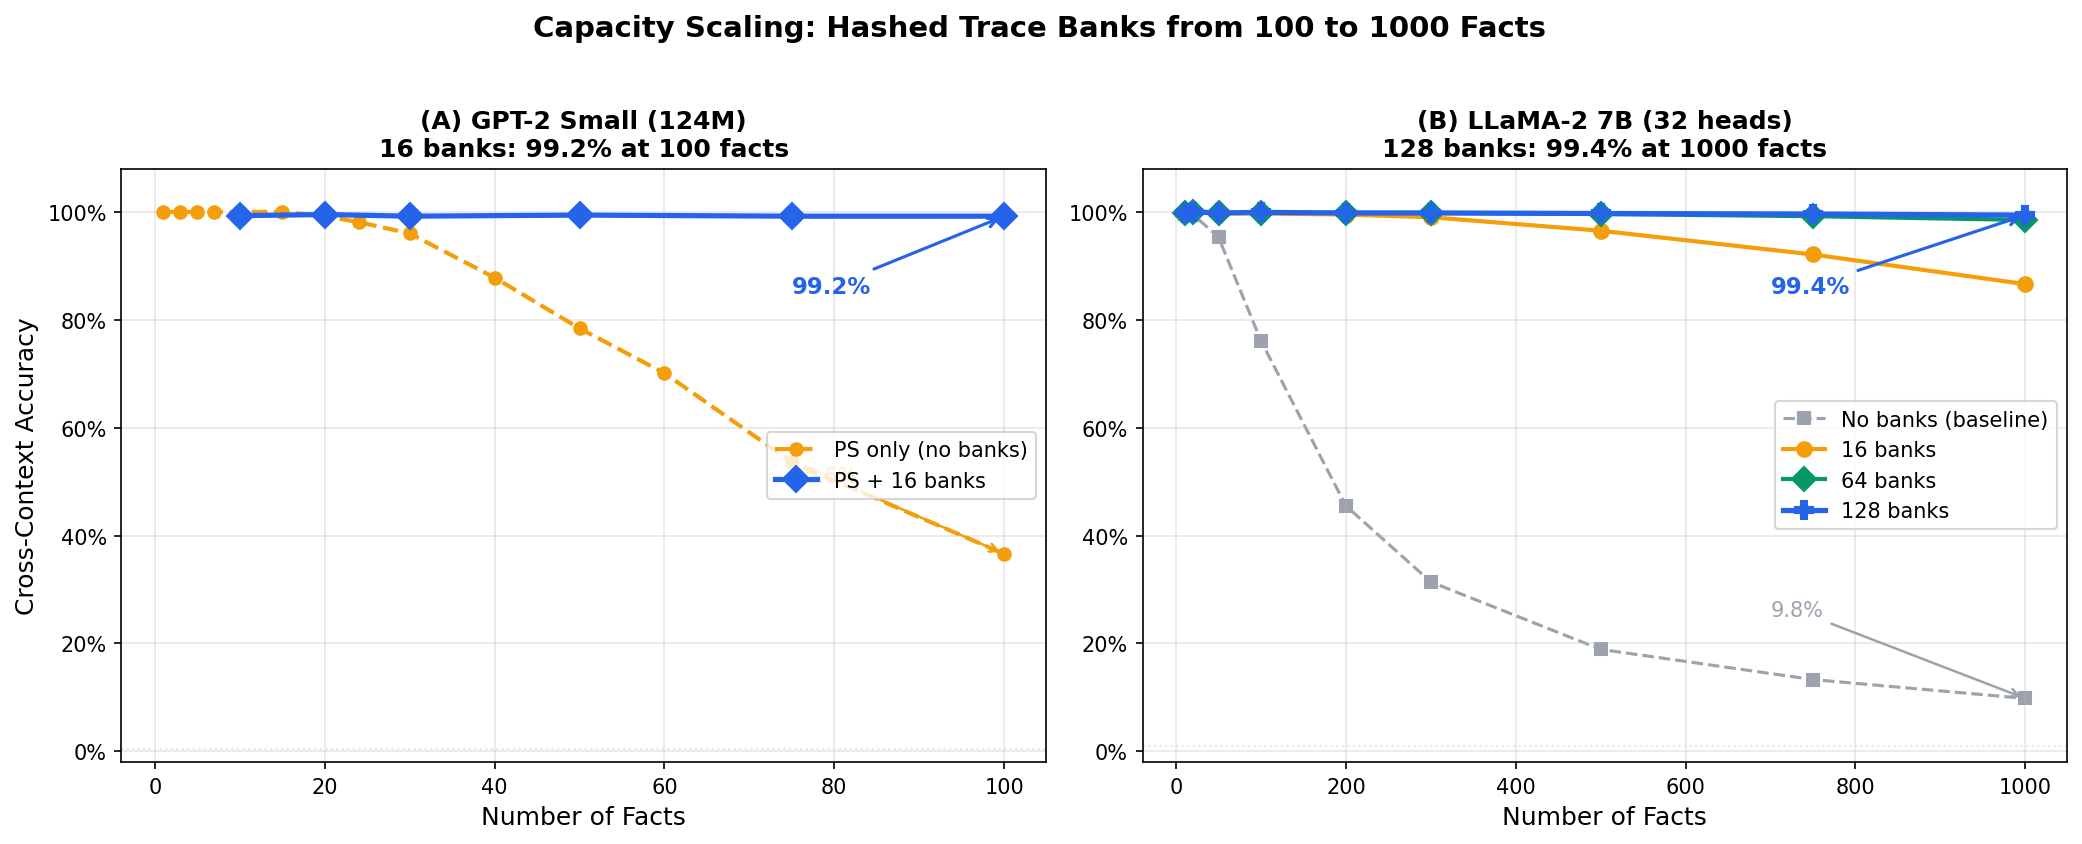
\includegraphics[width=\textwidth]{figures/capacity_curve.png}
    \caption{Capacity stress test. Without banks, pattern separation extends capacity to 95\% at $n{\approx}31$. With 16 hashed trace banks, accuracy remains ${\geq}99\%$ through $n{=}100$.}
    \label{fig:capacity}
  \end{subfigure}
  \hfill
  \begin{subfigure}[t]{0.48\textwidth}
    \centering
    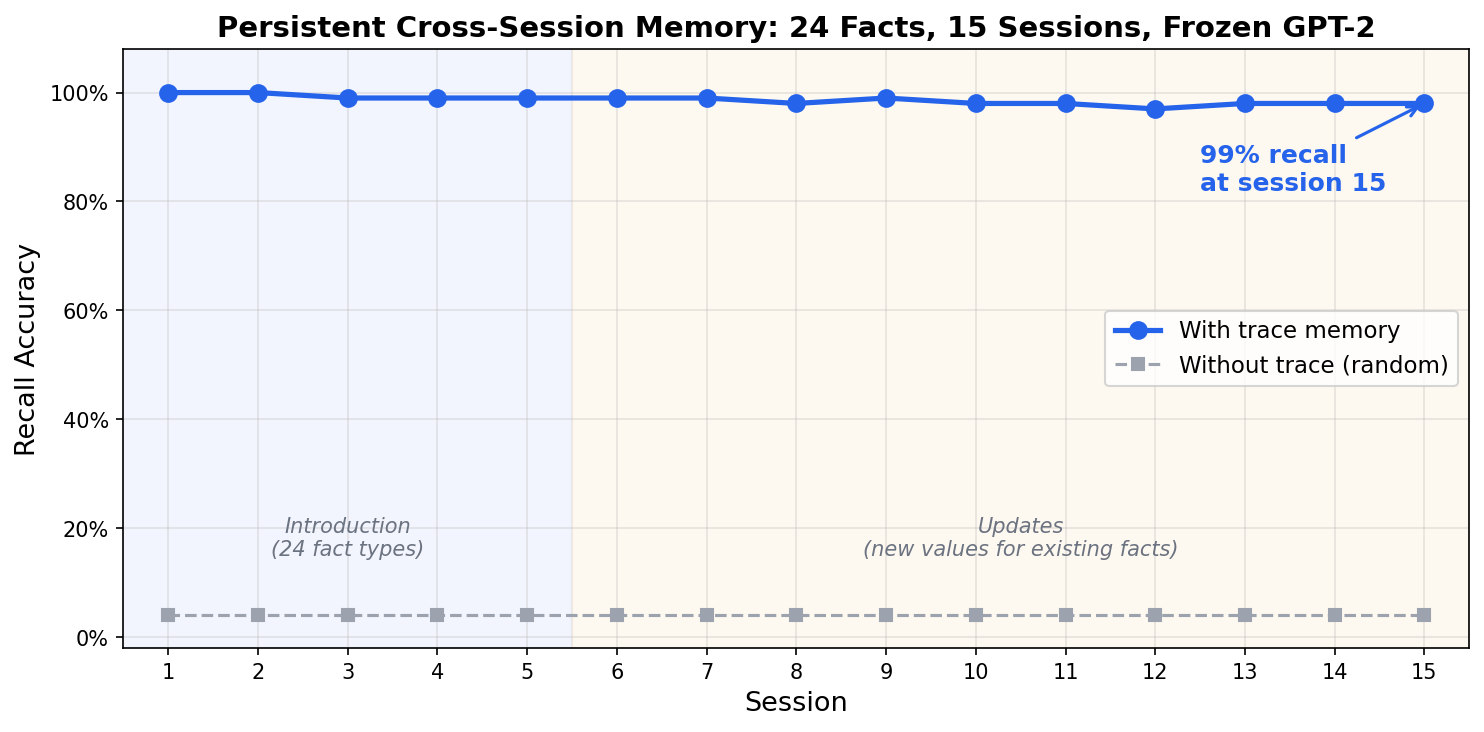
\includegraphics[width=\textwidth]{figures/retention_curve.png}
    \caption{Retention curve across 15 sessions. Recall remains ${\geq}97\%$ throughout, with ${\leq}2$pp drop from session~1 to session~15 despite ongoing fact updates.}
    \label{fig:retention}
  \end{subfigure}
  \caption{Capacity and retention characteristics of the Hebbian Trace Module on frozen GPT-2 Small.}
  \label{fig:capacity_retention}
\end{figure}

\subsection{Real-World Entity Vocabulary: LAMA T-REx}
\label{sec:lama}

To test storage capacity on realistic entity vocabularies beyond synthetic tasks, we evaluate on the LAMA T-REx benchmark \citep{petroni2019language}. We use LAMA as a source of real Wikidata facts with diverse entity tokens, rather than as an end-to-end knowledge probing test.

\textbf{Adaptation.}\quad LAMA facts are reformatted into the system's \texttt{\{concept\} \{linking\_token\} \{entity\}} templates, with each T-REx relation assigned a unique concept word. We evaluate two assignment strategies: (1)~\emph{oracle}: manually curated concept words optimized for single-token BPE and semantic precision (32 relations, 2,034 facts, 1,014 unique entity tokens), and (2)~\emph{auto}: concept words derived algorithmically from Wikidata property labels with zero manual curation (40 relations, 2,625 facts, 1,107 unique entity tokens). The auto algorithm splits each property label into words, removes stopwords, tries compound and individual words in deterministic order, and selects the first valid single-token BPE candidate, resolving collisions by falling back to the next candidate. Five collisions were resolved with semantically reasonable fallbacks (e.g., ``citizenship'' instead of ``country'' for P27); only one predicate (P36) was dropped. Random chance is ${\sim}0.1\%$.

\begin{table}[t]
  \centering
  \caption{LAMA T-REx evaluation: cross-context retrieval accuracy (100 episodes, bootstrap 95\% CIs). Oracle: 32 relations with manually curated concept words. Auto: 40 relations with concept words derived algorithmically from Wikidata property labels. Automated concept assignment achieves equivalent accuracy within CI, confirming that the trace does not depend on expert-selected addressing words.}
  \label{tab:lama}
  \begin{tabular}{@{}lcccc@{}}
    \toprule
    $n_{\text{facts}}$ & Oracle (32 rel) & Auto (40 rel) & In-context & No memory \\
    \midrule
    1  & \textbf{100.0\%}               & 99.0\%                      & 95.0\%  & 1.0\% \\
    3  & 94.0\% (91.3--96.3\%)          & \textbf{95.3\%} (93.0--97.3\%)  & 43.3\%  & 0.3\% \\
    5  & 93.8\% (91.6--95.8\%)          & \textbf{94.2\%} (92.2--96.0\%)  & 41.6\%  & 0.2\% \\
    7  & \textbf{88.7\%} (86.7--90.7\%) & 88.4\% (86.1--90.6\%)           & 29.7\%  & 0.3\% \\
    10 & 81.1\% (78.9--83.2\%)          & \textbf{83.9\%} (82.0--85.8\%)  & 24.7\%  & 0.1\% \\
    \bottomrule
  \end{tabular}
\end{table}

The trace exceeds the in-context baseline by +50--60pp at $n{\geq}3$ under both assignment strategies, demonstrating that Hebbian storage outperforms GPT-2's native in-context learning for structured fact retrieval on real-world knowledge. Automated concept assignment achieves accuracy within the confidence interval of oracle assignment at all fact counts, and slightly higher at $n{=}10$ (+2.8pp)---likely because more relations (40 vs.\ 32) provide greater entity diversity and reduce Q-collision between facts in the same episode.

\textbf{Scope.}\quad This evaluation tests the trace mechanism's associative storage capacity on real-world knowledge, not end-to-end knowledge probing. Each T-REx relation is mapped to a concept word (e.g., P36 $\to$ ``capital''), reducing the task to: store(``capital'', ``Paris''), query(``capital''). The LM is still needed---trace injection competes with GPT-2's pretrained prior---but concept-word assignment does not require expert curation. The single-token constraint limits coverage to ${\sim}6\%$ of LAMA T-REx entity tokens. These results validate storage capacity on real entity vocabularies (1,014--1,107 unique tokens vs.\ ${\sim}100$ in synthetic tasks), but do not demonstrate open-domain knowledge acquisition.

\subsection{Comparison with kNN-LM}
\label{sec:knn_comparison}

The kNN-LM \citep{khandelwal2020generalization} is the closest existing baseline: it attaches to a frozen LM, stores hidden states from fact passages, and interpolates nearest-neighbor retrieval with the LM distribution---all without fine-tuning. We implement kNN-LM with $k{=}32$, temperature $T{=}10$, interpolation weight $\lambda{=}0.25$ (tuned on a held-out sweep).

\begin{table}[t]
  \centering
  \caption{Hebbian trace vs.\ kNN-LM ($k{=}32$, $T{=}10$, $\lambda{=}0.25$). kNN-LM matches or exceeds the trace on LAMA (prefix-matching queries) but degrades toward the no-memory baseline on cross-context retrieval (different phrasing). 100 episodes, seed=42, GPT-2 Small with pattern separation.}
  \label{tab:knn}
  \begin{tabular}{@{}lccccc@{}}
    \toprule
    & \multicolumn{2}{c}{Cross-context (7 types)} & & \multicolumn{2}{c}{LAMA T-REx} \\
    \cmidrule{2-3} \cmidrule{5-6}
    $n$ & Trace & kNN-LM & & Trace & kNN-LM \\
    \midrule
    1  & \textbf{100.0\%} & 100.0\%       & & 100.0\% & 100.0\%       \\
    3  & \textbf{89.7\%}  & 37.0\%        & & 94.0\%  & 94.3\%        \\
    5  & \textbf{85.4\%}  & 22.4\%        & & 93.8\%  & \textbf{94.2\%} \\
    7  & \textbf{82.0\%}  & 14.9\%        & & 88.6\%  & \textbf{89.3\%} \\
    10 & ---               & ---           & & 81.4\%  & \textbf{82.9\%} \\
    \bottomrule
  \end{tabular}
\end{table}

Table~\ref{tab:knn} reveals a sharp dichotomy. The two benchmarks test fundamentally different properties: \emph{cross-context retrieval} measures whether a memory system can store a fact in one phrasing and retrieve it from another---a test of concept-addressed vs.\ contextual memory, not merely paraphrase robustness. \emph{LAMA} measures storage capacity on realistic entity vocabularies, but queries are exact prefixes of storage text (``capital is'' matches ``capital is Paris.''), so any system that memorizes hidden states can succeed.

On cross-context retrieval, kNN-LM degrades from 100\% at $n{=}1$ to 15\% at $n{=}7$ ($-67$pp vs.\ trace), approaching the no-memory baseline. On LAMA, kNN-LM \emph{matches or slightly exceeds} the trace (89\% vs.\ 89\% at $n{=}7$)---because prefix-matching queries produce identical hidden states under causal attention. The kNN-LM's slight advantage at higher $n$ reflects the fact that prefix matching gives zero-noise retrieval, while the trace's pattern separation introduces small Q-collision noise.

The mechanism behind this dichotomy is straightforward. kNN-LM uses contextual hidden states: the same fact stored in different phrasing produces different representations. When the query ``What is my name?'' differs from the storage ``My name is John.'', the hidden states diverge and nearest-neighbor retrieval fails. The Hebbian trace addresses via $\mathbf{Q}(\text{concept word})$ regardless of surrounding context, making storage and retrieval phrasing-invariant.

\textbf{Memory footprint.}\quad The trace stores a fixed $d_{\text{trace}}^2$ matrix per head per bank. For the GPT-2 Small configuration ($H{=}8$, $d_{\text{trace}}{=}64$, $B{=}16$ banks), this totals $64^2 \times 8 \times 16 = 524\text{K}$ parameters; for the LLaMA-2 7B configuration ($H{=}32$, $d_{\text{trace}}{=}64$, $B{=}128$ banks), $64^2 \times 32 \times 128 = 16.8\text{M}$ parameters---still only 0.24\% of the 7B model. Critically, this footprint is \emph{independent of the number of stored facts}: storing 10 or 1,000 facts requires the same memory. kNN-LM stores one $d_{\text{model}}$-dimensional vector per token position, growing as $O(N \cdot L)$ where $N$ is the number of facts and $L$ the average token length. At $n{=}1{,}000$ facts (${\sim}10{,}000$ tokens on LLaMA-2), kNN-LM requires ${\sim}40\text{M}$ floats ($4096 \times 10{,}000$)---$2.4\times$ the trace footprint and growing linearly. Retrieval cost also differs: the trace computes a single $\mathbf{Q} \times \mathbf{T}_v$ matrix-vector product ($O(d^2)$, constant per bank), while kNN-LM requires a nearest-neighbor search over all stored vectors ($O(N \cdot d)$, linear in datastore size).

\subsection{Pattern Completion via Autoassociative Trace}
\label{sec:tauto_exp}

Context-free addressing creates a fundamental limitation: paraphrased questions produce different Q-vectors than the concept word used during storage. ``What do people call you?'' generates Q(``call''), but the fact ``My name is John'' was stored at Q(``name''). Without correction, paraphrased queries score 17--24\% (near random).

\textbf{Setup.}\quad We define 17 Q$\to$Q template pairs mapping variant words to canonical concept words: Q(``I'')$\to$Q(``name''), Q(``home'')$\to$Q(``live''), Q(``employer'')$\to$Q(``work''), etc. These are written to $\mathbf{T}_{\text{auto}}$ once per episode.

\textbf{Results.}\quad Table~\ref{tab:tauto} shows dramatic improvements across query categories. Misaligned queries (shifted template position) improve from 18\% to 85\% at $n{=}5$, and semantic reformulations (entirely different phrasing) reach 100\% at all fact counts.

\begin{table}[t]
  \centering
  \caption{Pattern completion via $\mathbf{T}_{\text{auto}}$ (GPT-2 Small, $\alpha{=}0.5$, PS $8\times/k{=}16$, $\alpha_c{=}0.3$, 30 episodes). Aligned queries use the standard template; misaligned use shifted positions; semantic use entirely different phrasing.}
  \label{tab:tauto}
  \begin{tabular}{@{}ccccccc@{}}
    \toprule
    & \multicolumn{2}{c}{Aligned} & \multicolumn{2}{c}{Misaligned} & \multicolumn{2}{c}{Semantic} \\
    \cmidrule(lr){2-3} \cmidrule(lr){4-5} \cmidrule(lr){6-7}
    $n$ & Std & $+\mathbf{T}_{\text{auto}}$ & Std & $+\mathbf{T}_{\text{auto}}$ & Std & $+\mathbf{T}_{\text{auto}}$ \\
    \midrule
    1 & 100\% & 100\% & 17\% & \textbf{100\%} & 27\% & \textbf{100\%} \\
    3 & 100\% & 100\% & 22\% & \textbf{95\%} & 30\% & \textbf{100\%} \\
    5 & 100\% & 100\% & 19\% & \textbf{86\%} & 33\% & \textbf{100\%} \\
    7 & 100\% & 100\% & 24\% & \textbf{82\%} & 31\% & \textbf{100\%} \\
    \bottomrule
  \end{tabular}
\end{table}

\textbf{Cross-model scaling.}\quad On Phi-2 (2.7B), the same $\alpha_c{=}0.3$ is optimal---the completion-to-standard signal ratio is model-independent. Phi-2 achieves 95.3\% on misaligned queries at $n{=}5$ (vs.\ GPT-2's 90.7\%), with the advantage growing at higher fact counts (+7.3pp at $n{=}7$), confirming that richer embeddings improve two-step retrieval.

\textbf{Integration with full system.}\quad $\mathbf{T}_{\text{auto}}$ composes orthogonally with all existing mechanisms. In the 15-session flagship scenario with erasure, paraphrased queries on \emph{updated} facts return the \emph{new} value at 75\% accuracy---the completion channel correctly routes through the erased-and-rewritten $\mathbf{T}_v$.

\subsection{Multi-Hop Retrieval}
\label{sec:multihop_exp}

\textbf{Synthetic chains.}\quad We validate the multi-hop pipeline (Section~\ref{sec:multihop}) on 11 city$\to$country chain pairs (Moscow$\to$Russia, Paris$\to$France, etc.). Each episode stores person$\to$city facts via \texttt{write\_fact\_direct} plus city$\to$country chain links. The two-hop query retrieves the person's country.

\begin{table}[t]
  \centering
  \caption{Multi-hop chain accuracy (synthetic, 50--100 episodes, PS $8\times/k{=}16$). ``Total facts'' includes both standard person$\to$city facts and city$\to$country chain links.}
  \label{tab:multihop_synthetic}
  \begin{tabular}{@{}ccccl@{}}
    \toprule
    Total facts & Hop-1 & Hop-2$|$oracle & End-to-end & Notes \\
    \midrule
    12 & 100\% & 100\% & \textbf{100\%} & 1 standard + 11 chains \\
    17 & 100\% & 100\% & \textbf{100\%} & 5 standard + 11 chains + 1 extra \\
    27 & 100\% & 100\% & \textbf{100\%} & 15 standard + 11 chains + 1 extra \\
    32 & 89\% & 85\% & 74\% & Capacity limit \\
    \bottomrule
  \end{tabular}
\end{table}

Q-vector similarity between city tokens (mean cosine $= 0.188$ after pattern separation) confirms low cross-talk. Cross-group similarity between city and concept word Q-vectors is even lower (mean $= 0.091$), explaining why chain links and standard facts coexist without interference through 27 total facts.

\textbf{HotpotQA benchmark.}\quad We evaluate on real multi-hop questions from HotpotQA \citep{yang2018hotpotqa}, filtering the validation set to bridge-type questions with identifiable bridge entities and non-degenerate answers (bridge $\neq$ answer). Multi-token answers are evaluated via first BPE token match. Bridge entities are identified automatically from context paragraphs without oracle supporting facts. From 5,918 bridge questions, 4,159 pass all filters with auto bridge detection (vs.\ 4,876 with oracle annotations; 94.6\% bridge entity agreement on shared questions).

\begin{table}[t]
  \centering
  \caption{HotpotQA 2-hop evaluation (PS $8\times/k{=}16$, 32 banks). \textbf{Non-oracle}: bridge entities identified from context paragraphs (no supporting fact annotations); best-bank scan at retrieval (no oracle tokens). First BPE token answer match; not comparable to end-to-end QA leaderboard entries. Per-question: trace reset between questions. Batched: $N$ questions share a single trace, 50 random batches.}
  \label{tab:hotpotqa}
  \begin{tabular}{@{}ccccc@{}}
    \toprule
    Mode & $N$ & Total facts & E2E (no banks) & E2E (32 banks) \\
    \midrule
    Per-question & 1 & 2 & \textbf{100\%} (4,159/4,159) & \textbf{100\%} \\
    \midrule
    Batched & 5 & 10 & 98.0\% & \textbf{100\%} \\
    Batched & 8 & 16 & 94.5\% & \textbf{99.5\%} \\
    Batched & 10 & 20 & 88.2\% & \textbf{98.8\%} \\
    Batched & 15 & 30 & 62.7\% & \textbf{98.7\%} \\
    \bottomrule
  \end{tabular}
\end{table}

The primary bottleneck without banks is bridge-entity first-token collision, creating identical Q-vectors at hop-2. Hashed trace banks (Section~\ref{sec:banks}) resolve this: with 32 banks and a best-bank scan at retrieval (reading all banks and selecting the highest-confidence answer), end-to-end accuracy improves from 62.7\% to 98.7\% at batch size 15 (+36pp). Oracle bridge detection yields comparable results (97.5\% at batch 15 on 4,876 questions with 32 banks), confirming that auto detection introduces no meaningful accuracy loss. Notably, modifying the Q-vector itself (composite Q from multiple entity tokens) is incompatible with pattern separation's top-k sparsification---even tiny perturbations change which expanded dimensions survive top-k, breaking write/read address alignment. Banks solve the collision without altering Q, preserving pattern separation compatibility.

We emphasize that this evaluation tests the trace mechanism's multi-hop capability on real-world facts, not end-to-end QA performance---first-token answer matching means these results are not directly comparable to HotpotQA leaderboard entries, which must additionally solve retrieval from 5M+ paragraphs and open-ended answer generation.

\subsection{Free-Text Pipeline and Dialogue Integration}
\label{sec:freetext}

The preceding experiments use structured templates. We validate the path toward natural interaction through three extensions.

\textbf{Free-text extraction.}\quad A direct-write API (\texttt{write\_fact\_direct}) bypasses the template machinery entirely, storing associations via \texttt{compute\_q\_for\_token} and \texttt{compute\_v\_for\_token}. A regex-based extractor identifies concept--entity pairs from free-form utterances (``I live in Paris'', ``Call me John'', ``My favorite color is blue'') with 100\% precision and 94.1\% recall. End-to-end accuracy matches the template pipeline (80.8\% at $n{=}5$), confirming zero overhead from the direct-write path.

\textbf{LLM-based extraction.}\quad We replace the regex extractor with Flan-T5-small (80M parameters), a lightweight sequence-to-sequence model that performs per-type extractive QA (e.g., ``What is the person's name?''). Dual validation---entity must appear in both the concept vocabulary pool and the source text---prevents hallucination false positives. On unconstrained free-form text where regex extraction achieves 0\% F1 (e.g., ``After years abroad, Alice settled in Paris and found a job at Google''), the LLM extractor achieves 94\% F1. Overall across all text tiers: oracle 100\%, LLM 93.9\%, regex 77.4\%. End-to-end trace accuracy with LLM extraction matches or slightly exceeds regex across all fact counts, confirming that the trace mechanism is format-agnostic---the bottleneck was extraction, not storage.

\textbf{Multi-turn dialogue.}\quad Facts accumulate across dialogue turns. 10 dialogue templates across 3 categories (introduction, update, dense) test natural conversation flow. Results: 100\% across all phases---introduction (1,400 queries), updates with erasure (1,200 queries including 250 updated facts), and multi-dialogue sessions (5 dialogues, ${\sim}10$ accumulated facts). The erasure mechanism handles in-dialogue corrections (``Actually, I moved to London'') with 100\% accuracy.

% ============================================================
\section{Discussion}

\subsection{Composability as a Design Principle}

A central finding is that bio-inspired mechanisms compose orthogonally when they target independent bottlenecks. Pattern separation reduces storage interference; gating reduces input noise; erasure handles updates; CLS decay manages temporal dynamics; $\mathbf{T}_{\text{auto}}$ resolves query variants; and multi-hop chains extend retrieval depth. No component interferes with another, and their benefits are approximately additive. The 15-session flagship with $\mathbf{T}_{\text{auto}}$ demonstrates the strongest composition test: seven mechanisms operating simultaneously (DG, CA3-hetero, CA3-auto, ACh gates, reconsolidation, CLS, replay) maintain 98\% standard recall while adding paraphrase resolution at 75\% on updated facts. This suggests that the hippocampal memory system's multi-mechanism architecture is not merely an evolutionary accident but a functionally optimal decomposition.

\subsection{Logit-Space Injection as a Universal Memory Interface}

A key architectural decision is injecting retrieved information at the logit level (Equation~\ref{eq:logit_injection}) rather than into intermediate hidden states. This choice is motivated by a practical observation: GPT-2's residual stream norms reach ${\sim}3{,}000$ in late layers, while the trace module's output norms are ${\sim}0.06$---a $50{,}000\times$ scale mismatch that makes hidden-state injection ineffective without layer-specific calibration. Logit-space injection sidesteps this entirely: the trace output is projected through the model's own embedding matrix $\mathbf{W}_{\text{embed}}^\top$, producing a bias in the vocabulary distribution that is naturally calibrated regardless of model scale.

This design has three consequences that extend beyond our specific system. First, it enables \emph{model-agnostic attachment}---the same trace module transfers from GPT-2 (124M) to LLaMA-2 (7B) without recalibration beyond $\alpha$, because logit space is anchored to the shared vocabulary. Second, it preserves the frozen model's distribution: trace injection shifts token probabilities without corrupting learned representations. Third, it provides a clean separation of concerns---the base model handles language generation while the trace module handles factual recall, composing at the output level rather than entangling in hidden dynamics. We suggest that logit-space injection may serve as a general interface for external memory modules attached to frozen language models.

\subsection{Positioning Relative to RAG and Fine-Tuning}

The Hebbian Trace Module occupies a distinct niche in the design space of LLM memory augmentation. Table~\ref{tab:positioning} compares the trace with two dominant approaches---retrieval-augmented generation (RAG) and parameter fine-tuning---along five axes relevant to practitioners.

\begin{table}[t]
  \centering
  \caption{Design-space comparison of memory augmentation approaches for LLMs. ``Organic updates'' refers to the ability to incrementally store new information at inference time without re-indexing or retraining.}
  \label{tab:positioning}
  \begin{tabular}{@{}lccc@{}}
    \toprule
    Property & Hebbian Trace & RAG & Fine-tuning \\
    \midrule
    Modifies model weights     & No  & No  & Yes \\
    External infrastructure    & None & Vector DB + indexing & Training pipeline \\
    Organic incremental updates & Yes (Hebbian write) & No (re-index) & No (retrain) \\
    Cross-session persistence  & Yes (trace serialization) & Yes (datastore) & Yes (weights) \\
    Retrieval cost              & $O(d^2)$ constant & $O(N \cdot d)$ or $O(\log N)$ & $O(1)$ (amortized) \\
    Capacity (current)         & ${\sim}1{,}000$ facts (${\geq}99\%$) & $10^6$+ documents & Unbounded \\
    Phrasing invariance        & Yes (context-free Q) & Partial (embedding similarity) & Yes (parametric) \\
    \bottomrule
  \end{tabular}
\end{table}

The trace's primary advantages are \emph{zero infrastructure}---no vector database, indexing pipeline, or training loop---and \emph{organic updates}: new facts are written via a single Hebbian outer product at inference time, with no re-indexing or gradient computation. Context-free addressing provides phrasing-invariant retrieval that RAG systems achieve only partially through embedding similarity, which degrades when query and document phrasing diverge substantially (as demonstrated by the +63pp advantage over kNN-LM on cross-context retrieval).

The trace's primary disadvantage is \emph{capacity}. At ${\sim}1{,}000$ facts with ${\geq}99\%$ accuracy (128 hashed banks, LLaMA-2 7B), the current system covers a substantial range of personal knowledge management---user preferences, biographical facts, interaction history, work context---but cannot replace RAG for large-scale document retrieval or fine-tuning for broad knowledge integration. Crucially, this capacity comes at zero latency overhead: bank routing adds $<0.1$ms to the ${\sim}17$ms LM forward pass (Table~\ref{tab:latency}). This positions the trace as complementary to, rather than a replacement for, existing approaches: it handles the fast-changing, user-specific ``episodic'' layer of memory that RAG and fine-tuning address poorly, while those systems handle the ``semantic'' layer of large-scale world knowledge.

A practical deployment might combine all three: the trace for per-user facts accumulated during interaction, RAG for organizational knowledge bases, and the frozen pretrained model for general world knowledge---mirroring the hippocampal (fast/episodic), neocortical (slow/semantic), and genetic (innate/parametric) memory systems of biological organisms.

\subsection{Limitations}

We identify five concrete limitations, noting where recent extensions have partially addressed them:

\begin{enumerate}[leftmargin=*]
  \item \textbf{Structured input dependency (largely addressed).} The core trace mechanism is format-agnostic---it requires only (concept\_token\_id, entity\_token\_id) pairs. The LLM-based extraction pipeline (Section~\ref{sec:freetext}) achieves 94\% F1 on unconstrained free-form text where regex extraction fails entirely, demonstrating that the bottleneck was extraction, not storage. Remaining gaps include ambiguous references (``The red one has always been my favorite'') where entity identity requires discourse-level reasoning beyond single-utterance QA.

  \item \textbf{Single-token entities (largely addressed).} Entity values must tokenize to exactly one BPE token. Multi-hop chains use first-token addressing for multi-token bridge entities (Section~\ref{sec:multihop_exp}), which produces collisions. Hashed trace banks with best-bank scan resolve these collisions (+36pp at batch 15, maintaining ${\geq}98.7\%$ accuracy), but direct multi-token Q addressing remains incompatible with pattern separation's top-k step.

  \item \textbf{Context-free addressing trade-off.} Using token identity for addressing enables cross-session stability but cannot distinguish ``my name'' from ``Alice's name''. $\mathbf{T}_{\text{auto}}$ partially mitigates the related paraphrase problem, but the ownership-discrimination Pareto trade-off (Section~\ref{sec:context_enriched}) remains unresolved.

  \item \textbf{Capacity scaling (largely addressed).} Hashed trace banks extend capacity to ${\geq}99\%$ at $n{=}1{,}000$ simultaneously stored facts on LLaMA-2 7B with 128 banks (vs.\ 9.8\% baseline), with zero measurable latency overhead (Table~\ref{tab:latency}). The degradation rate at 128 banks ($-0.3$pp per 500 facts from $n{=}500$ to $n{=}1{,}000$) suggests the capacity knee lies beyond $n{\approx}2{,}000$, though this has not been verified experimentally. For applications requiring $10{,}000$+ facts, the current best-bank scan (reading all $B$ banks per query) would need to be replaced by hierarchical or learned bank routing to avoid $O(B)$ retrieval cost. Additionally, the scaling behavior across model architectures remains uneven: while LLaMA-2 7B achieves near-perfect scaling, Mistral 7B ($\alpha{=}1000$ vs.\ $\alpha{=}10$ for LLaMA-2 at the same $d_{\text{model}}$) does not benefit from head scaling, suggesting model-specific embedding geometry incompatibilities that require further investigation.

  \item \textbf{Benchmark coverage (largely addressed).} The HotpotQA evaluation (4,159 bridge questions with non-oracle detection, Section~\ref{sec:multihop_exp}) covers the majority of bridge-type questions via first-token answer matching. Auto bridge detection (from context paragraphs, no supporting fact annotations) achieves 94.6\% agreement with oracle annotations and equivalent accuracy with banks. The remaining gap to end-to-end QA involves open retrieval from 5M+ paragraphs and open-ended answer generation, which are outside the scope of the trace mechanism itself.
\end{enumerate}

\subsection{Connection to Biological Memory}

Our architecture implements a simplified hippocampal loop: dentate gyrus (pattern separation) $\to$ CA3 (Hebbian trace) $\to$ cholinergic modulation (dual gates) $\to$ reconsolidation (erasure). We do not claim biological fidelity---rather, we use neuroscience as a source of architectural inductive biases that prove empirically effective. The consistent success of these biases across five model scales and four distinct architectures (GPT-2, Phi-2, LLaMA-2, Mistral) suggests that the computational principles underlying hippocampal memory are relevant beyond biological neural networks.

% ============================================================
\section{Future Work}

Several directions extend from the current foundation:

\textbf{Open-domain relation types.}\quad The LLM-based extractor (Section~\ref{sec:freetext}) currently operates over a fixed concept vocabulary of 24 types. Extending to open-domain relation types---where the LLM identifies both the relation and entity from arbitrary text---would remove the last vocabulary constraint. This requires structured key addressing (e.g., \texttt{capital\_of(France)} $\to$ \texttt{Paris} rather than \texttt{capital} $\to$ \texttt{Paris}) to prevent collisions across relation instances.

\textbf{Multi-token entity addressing.}\quad First-token addressing produces collisions for common BPE prefixes. Hash-routed trace banks with best-bank scan already resolve these collisions (Table~\ref{tab:hotpotqa}), but direct Q-space addressing from multiple tokens remains an open problem: composite Q (blending or perturbing Q-vectors from entity tokens) is incompatible with pattern separation's top-k sparsification, as even small perturbations change which expanded dimensions survive the top-k step.

\textbf{Episodic memory for agents.}\quad The current system stores declarative facts. Extending trace to store experiential episodes---situation-action-outcome tuples---would enable inference-time learning for LLM-based agents, where performance improves across episodes without weight updates.

\textbf{Neocortical consolidation.}\quad In biological memory, hippocampal traces are gradually consolidated into neocortical representations. An analog process---periodically distilling trace contents into model weights through targeted fine-tuning---could combine the fast learning of Hebbian traces with the capacity of parametric memory.

\textbf{Model-specific embedding geometry.}\quad Mistral 7B requires $\alpha{=}1000$ (vs.\ $\alpha{=}10$ for LLaMA-2 at the same $d_{\text{model}}{=}4096$) and does not benefit from trace head scaling, suggesting a fundamentally different embedding geometry. Investigating whether Mistral's embedding structure (e.g., norm distributions, cosine similarity patterns, or the effect of grouped-query attention on trace-relevant subspaces) requires architectural adaptation---such as learned $\mathbf{W}_{\text{out}}$ or model-specific $d_{\text{trace}}$ selection---would establish the boundary conditions for zero-shot trace transfer.

% ============================================================
\section{Conclusion}

We have presented the Hebbian Trace Module, an external memory system that provides persistent, updatable, and compositional knowledge retention for frozen language models. The core architectural insight is that hippocampal memory principles---sparse pattern separation, Hebbian association, gated encoding, reconsolidation, and complementary learning rates---translate into composable computational mechanisms that each address an independent bottleneck. Systematic ablation confirms that these mechanisms combine orthogonally, and their transfer across five model scales (124M to 7B) and three tokenizer families suggests that the underlying computational principles generalize beyond any single architecture.

Two results carry particular significance for the broader field. First, context-free addressing---using token identity rather than contextual hidden states---enables genuine cross-context retrieval where storage and query phrasing differ, a capability absent from nearest-neighbor approaches like kNN-LM (+63pp advantage). Second, logit-space injection provides a model-agnostic interface that requires only $\alpha$ calibration to transfer across architectures, suggesting a general pattern for external memory attachment.

Significant limitations remain. The single-token entity constraint and fixed concept vocabulary restrict the current system to structured fact types. However, capacity---previously the primary bottleneck---scales to 1,000 simultaneous facts at ${\geq}99\%$ accuracy via 128 hashed trace banks on LLaMA-2 7B, with zero latency overhead, and degradation trends suggest the knee extends beyond 2,000 facts. The HotpotQA evaluation validates multi-hop retrieval on 4,159 real-world questions without oracle support, though first-token answer matching means the results are not directly comparable to end-to-end QA systems. These constraints position the trace as complementary to RAG and fine-tuning---handling the fast-changing, user-specific episodic layer that those approaches address poorly---rather than as a replacement.

Nevertheless, our results demonstrate that persistent, compositional memory can be added to pretrained language models as a modular plug-in, without modifying model weights, at a fraction of the base model's parameter count. The consistent effectiveness of biologically motivated inductive biases across diverse architectures suggests that the computational principles underlying hippocampal memory offer a productive design vocabulary for machine learning systems that must learn incrementally at inference time.

% ============================================================
\bibliography{references}

\end{document}